\documentclass{article}
\usepackage{amsmath}
\usepackage{amssymb}
\usepackage{tikz}
\usetikzlibrary{calc}

\begin{document}

\begin{figure}[h]
    \centering
    \begin{tikzpicture}[scale=1.5]
        % Define points
        \coordinate (A) at (-2,0);
        \coordinate (B) at (0,0);
        \coordinate (C) at (2,0);
        \coordinate (D) at (3,1);
        \coordinate (E) at (4,1);
        \coordinate (F) at (5,1);
        \coordinate (G) at (6,1);
        \coordinate (H) at (7,1);
        \coordinate (I) at (8,1);
        \coordinate (J) at (9,1);
        \coordinate (K) at (10,1);
        \coordinate (L) at (11,1);
        \coordinate (M) at (12,1);
        \coordinate (N) at (13,1);
        \coordinate (O) at (14,1);
        \coordinate (P) at (15,1);
        \coordinate (Q) at (16,1);
        \coordinate (R) at (17,1);
        \coordinate (S) at (18,1);
        \coordinate (T) at (19,1);
        \coordinate (U) at (20,1);
        \coordinate (V) at (21,1);
        \coordinate (W) at (22,1);
        \coordinate (X) at (23,1);
        \coordinate (Y) at (24,1);
        \coordinate (Z) at (25,1);
        
        % Draw curves
        \draw[thick] (A) .. controls (B) and (C) .. (D);
        \draw[thick] (E) -- (F);
        \draw[thick] (G) -- (H);
        \draw[thick] (I) -- (J);
        \draw[thick] (K) -- (L);
        \draw[thick] (M) -- (N);
        \draw[thick] (O) -- (P);
        \draw[thick] (Q) -- (R);
        \draw[thick] (S) -- (T);
        \draw[thick] (U) -- (V);
        \draw[thick] (W) -- (X);
        \draw[thick] (Y) -- (Z);
        
        % Draw dashed lines
        \draw[dashed] (F) -- (G);
        \draw[dashed] (H) -- (I);
        \draw[dashed] (J) -- (K);
        \draw[dashed] (L) -- (M);
        \draw[dashed] (N) -- (O);
        \draw[dashed] (P) -- (Q);
        \draw[dashed] (R) -- (S);
        \draw[dashed] (T) -- (U);
        \draw[dashed] (V) -- (W);
        \draw[dashed] (X) -- (Y);
        \draw[dashed] (Z) -- (A);
        
        % Mark points
        \filldraw[black] (B) circle (1pt) node[anchor=south] {$u_t$};
        \filldraw[black] (D) circle (1pt) node[anchor=south] {$\bar{u}_{t+1}$};
        \filldraw[black] (F) circle (1pt) node[anchor=south] {$u_t - P_t^n g_t$};
        \filldraw[black] (G) circle (1pt) node[anchor=south] {$u_t - g_t$};
        
        % Labels
        \node at (1,2) {$\mathcal{M}$};
        \node at (15,2) {$\mathcal{T}_t$};
    \end{tikzpicture}
    \caption{Illustration of the proposed algorithm: based on an iterate $u_t \in \mathcal{M}$ and the choice of a linear space $\mathcal{T}_t$, an approximation $P_t^n g_t \in \mathcal{T}_t$ of the true gradient $g_t$ is first obtained via a random operator $P_t^n$. Then an update $\bar{u}_{t+1} = u_t - s_t P_t^n g_t$ is obtained given a step size $s_t$. Then, the next iterate $u_{t+1} \in \mathcal{M}$ is obtained through application of the retraction map $R_t$.}
    \label{fig:algorithm_illustration}
\end{figure}

\end{document}